%%======%%======%0%======%%=======%%
\vspace{5mm}
\section{Compatibilidade de dispositivo}
%%======%%======%0%======%%=======%%

Além da compatibilidade por dimensionamento de tela, ainda é necessário averiguar o funcionamento do \textit{website} em diferentes navegadores, e eventualmente diferentes sistemas operacionais. 

\subsection{Teste de compatibilidade entre navegadores}

A compatibilidade deve ser verificada nos navegadores Google Chrome, Firefox, Edge, Safari e Brave.

Os fluxos principais a serem executados incluem a navegação entre páginas, utilização dos filtros do repositório, abertura dos equipamentos, utilização dos formulários, login, troca de idioma, alteração do tema e utilização do menu em telas menores.

\begin{table}[H]
	\centering
	\caption{Resultados dos testes de compatibilidade entre navegadores.}
	\label{tab:compatibilidade-navegadores}
	\renewcommand{\arraystretch}{1.4}
	\setlength{\tabcolsep}{9pt}
	\begin{tabular}{lcccccc}
		\hline
		\textbf{Fluxo testado} &
		\textbf{Chrome} &
		\textbf{Edge} &
		\textbf{Firefox} &
		\textbf{Safari} &
		\textbf{Brave} &
		\textbf{Opera} \\
		\hline
		Navegação entre páginas & $\checkmark$ & $\checkmark$ & $\checkmark$ & $\checkmark$ & $\checkmark$ & $\checkmark$ \\
		Filtros do repositório & $\checkmark$ & $\checkmark$ & $\checkmark$ & $\checkmark$ & $\checkmark$ & $\checkmark$ \\
		Abertura dos equipamentos & $\checkmark$ & $\checkmark$ & $\checkmark$ & $\checkmark$ & $\checkmark$ & $\checkmark$\\
		Formulários & $\checkmark$ & $\checkmark$ & $\checkmark$ & $\checkmark$ & $\checkmark$ & $\checkmark$ \\
		Login & $\checkmark$ & $\checkmark$ & $\checkmark$ & $\checkmark$ & $\checkmark$ & $\checkmark$ \\
		Troca de idioma & $\checkmark$ & $\checkmark$ & $\checkmark$ & $\checkmark$ & $\checkmark$ & $\checkmark$\\
		Alteração do tema & $\checkmark$ & $\checkmark$ & $\checkmark$ & $\checkmark$ & $\checkmark$ & $\checkmark$\\
		Menu em telas menores & $\checkmark$ & $\checkmark$ & $\checkmark$ & $\checkmark$ & $\checkmark$ & $\checkmark$\\
		\hline
	\end{tabular}
\end{table}

\begin{figure}[H]
	\centering
	
	\begin{subfigure}[t]{0.30\textwidth}
		\centering
		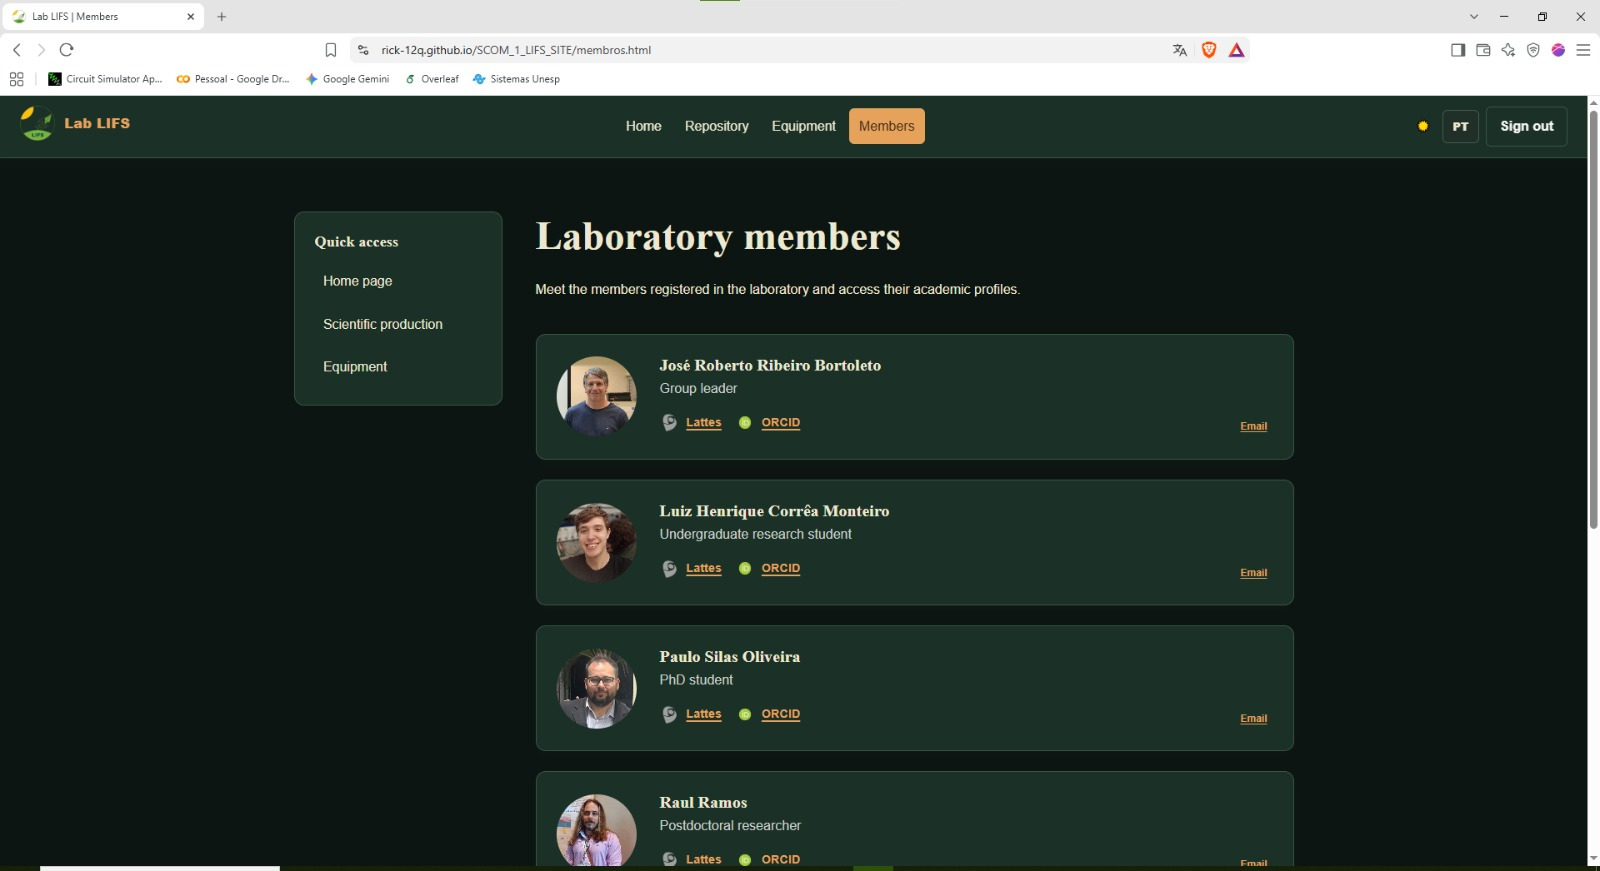
\includegraphics[width=\linewidth,height=0.23\textheight,keepaspectratio]{2-imagens/brave}
		\caption{Brave}
		\label{fig:brave}
	\end{subfigure}
	\hfill
	\begin{subfigure}[t]{0.30\textwidth}
		\centering
		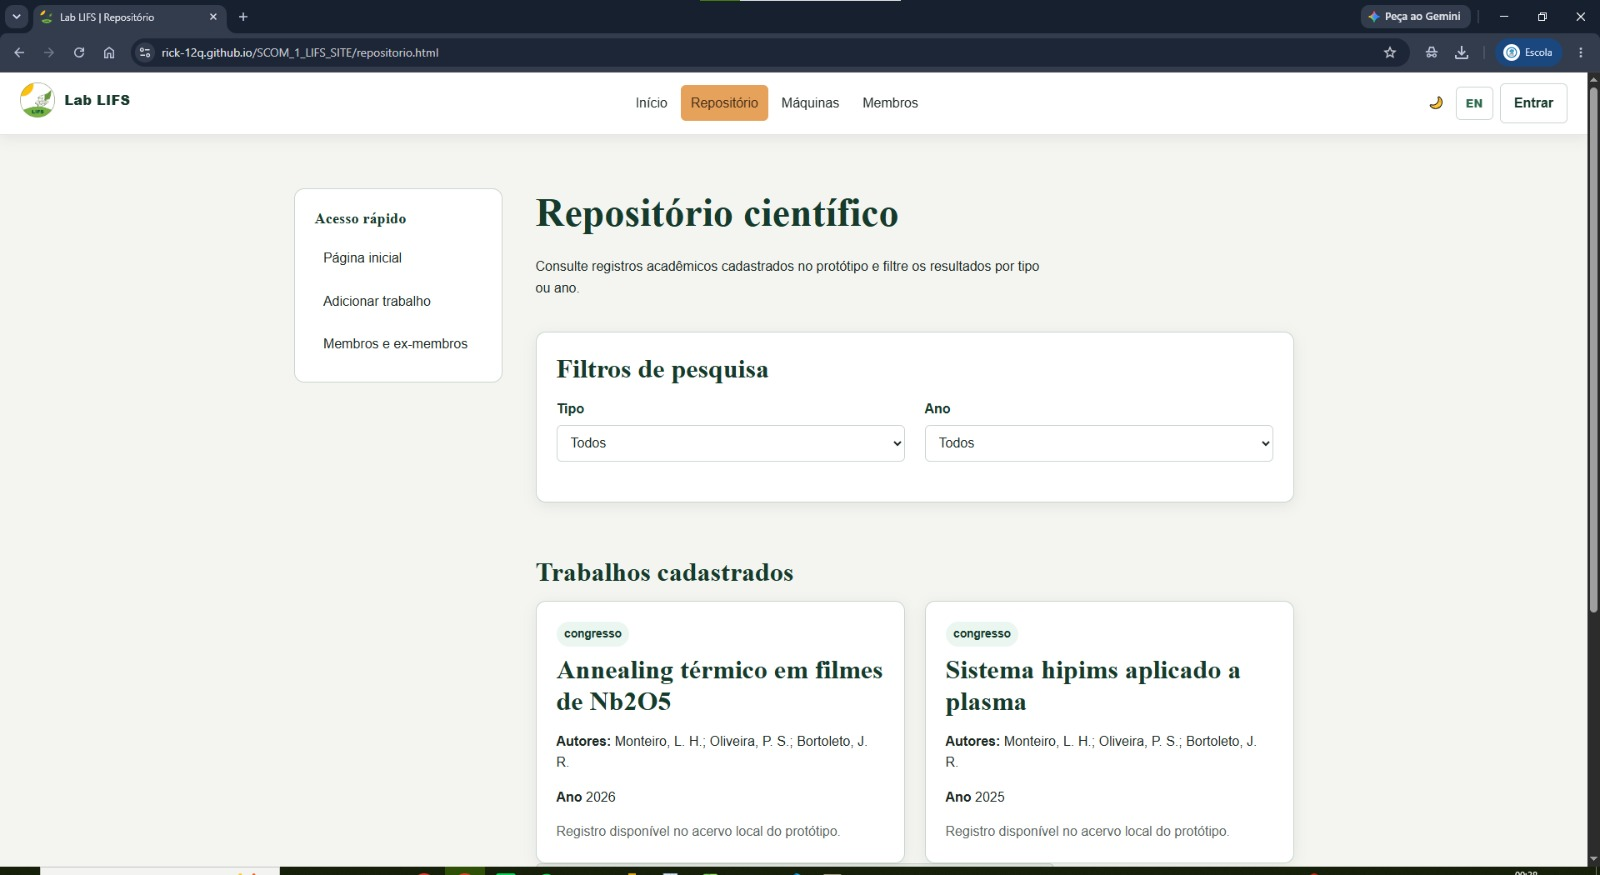
\includegraphics[width=\linewidth,height=0.23\textheight,keepaspectratio]{2-imagens/google}
		\caption{Google Chrome}
		\label{fig:google}
	\end{subfigure}
	\hfill
	\begin{subfigure}[t]{0.30\textwidth}
		\centering
		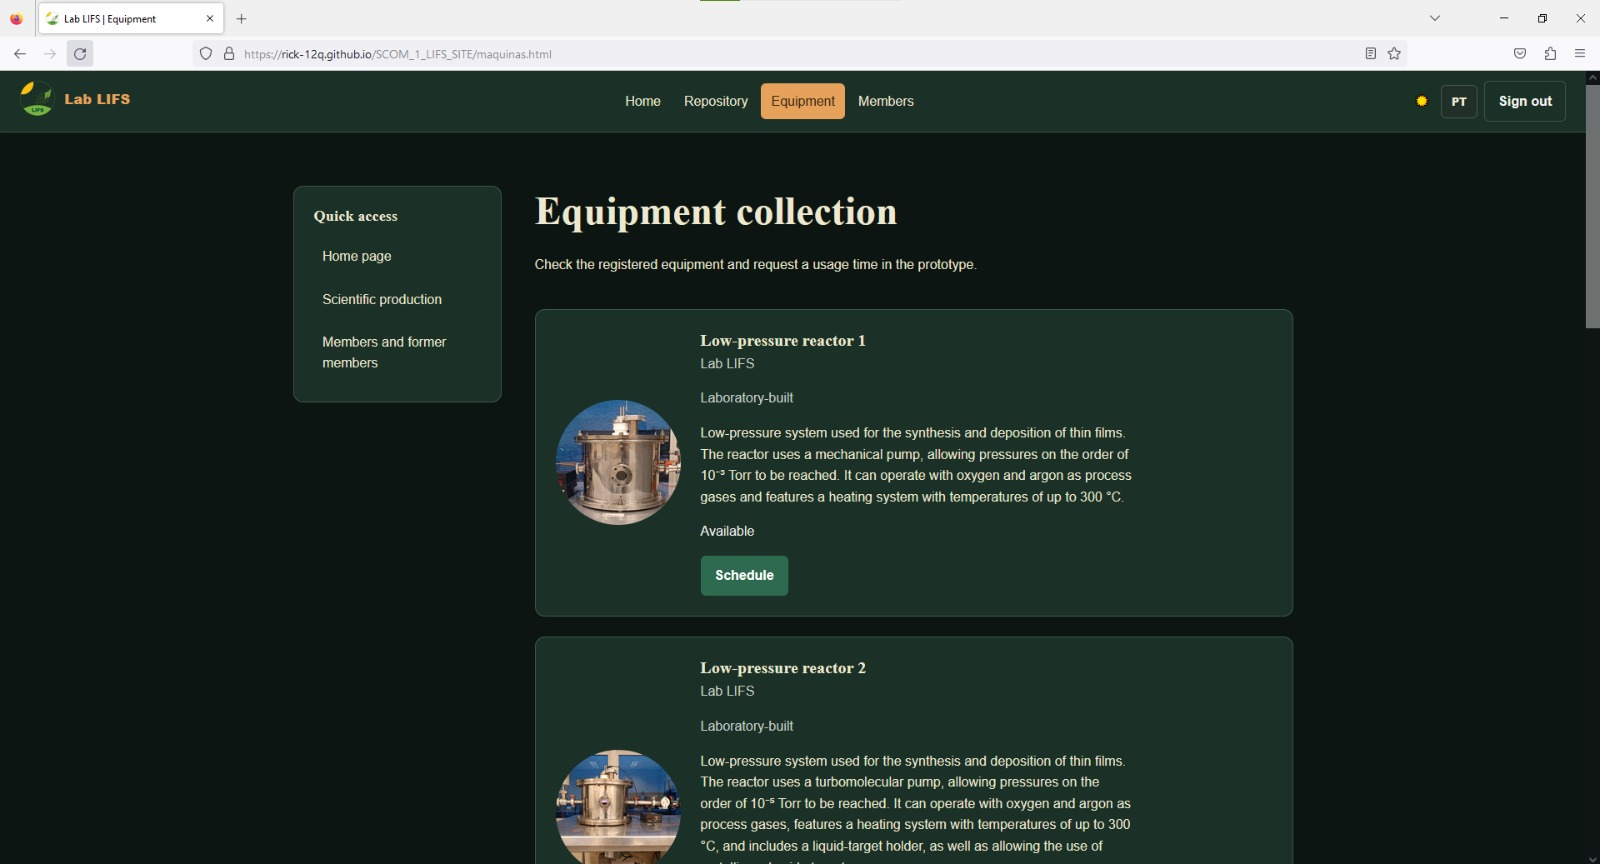
\includegraphics[width=\linewidth,height=0.23\textheight,keepaspectratio]{2-imagens/firefox}
		\caption{Mozilla Firefox}
		\label{fig:firefox}
	\end{subfigure}
	
	\vspace{8mm}
	
	\begin{subfigure}[t]{0.30\textwidth}
		\centering
		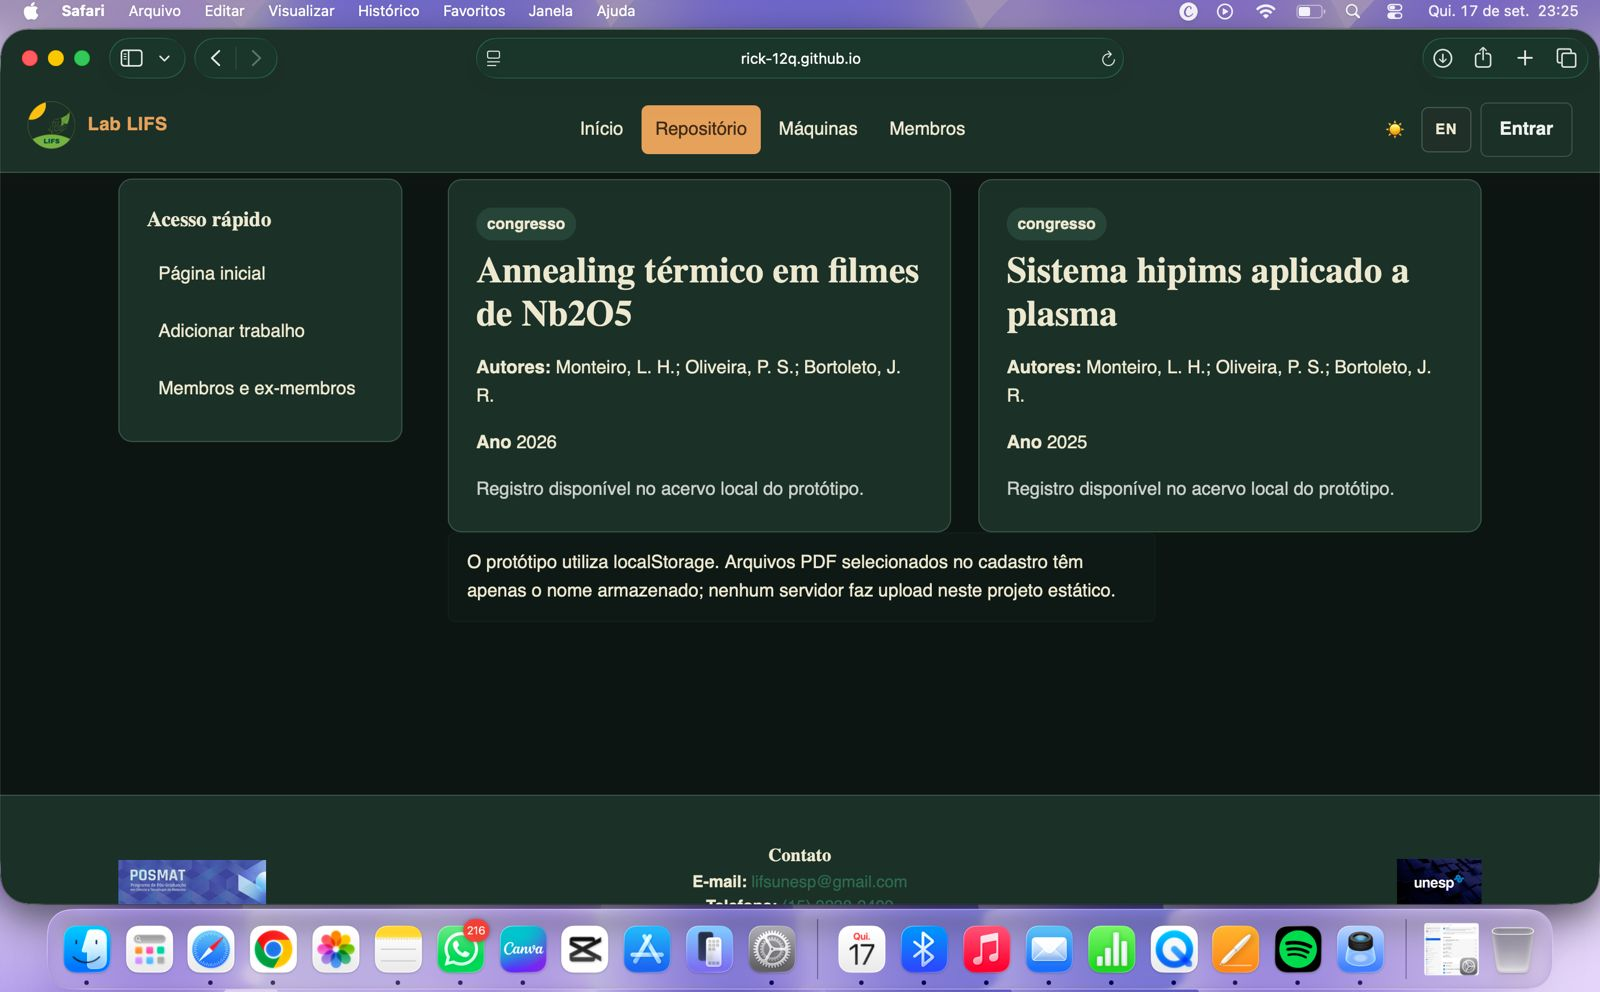
\includegraphics[width=\linewidth,height=0.23\textheight,keepaspectratio]{2-imagens/safari}
		\caption{Safari}
		\label{fig:safari}
	\end{subfigure}
	\hfill
	\begin{subfigure}[t]{0.30\textwidth}
		\centering
		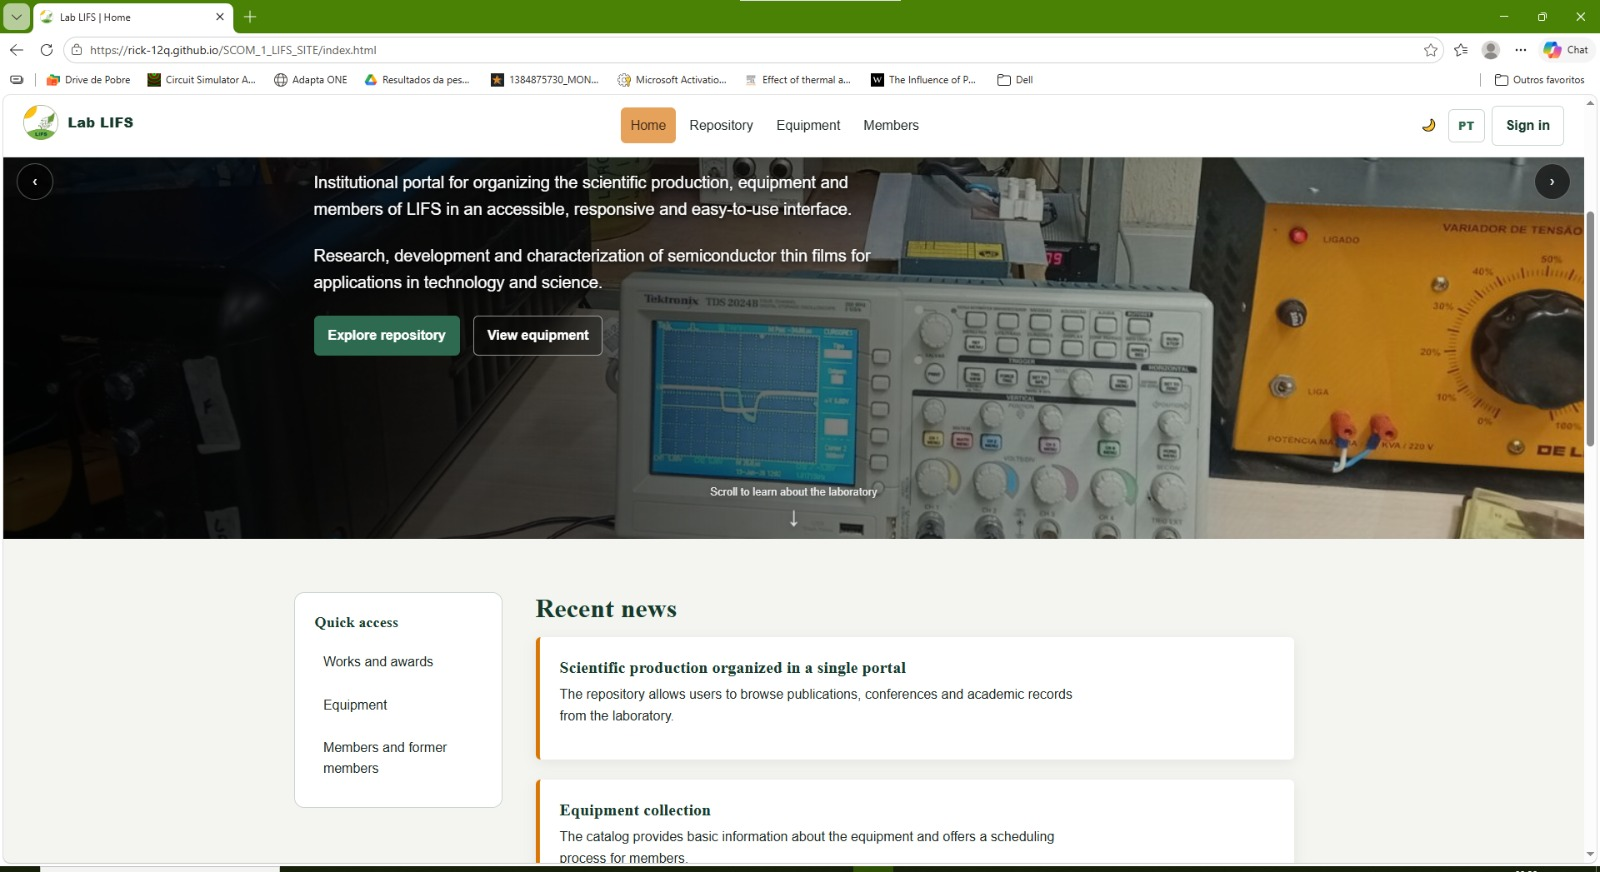
\includegraphics[width=\linewidth,height=0.23\textheight,keepaspectratio]{2-imagens/edge}
		\caption{Microsoft Edge}
		\label{fig:edge}
	\end{subfigure}
	\hfill
	\begin{subfigure}[t]{0.30\textwidth}
		\centering
		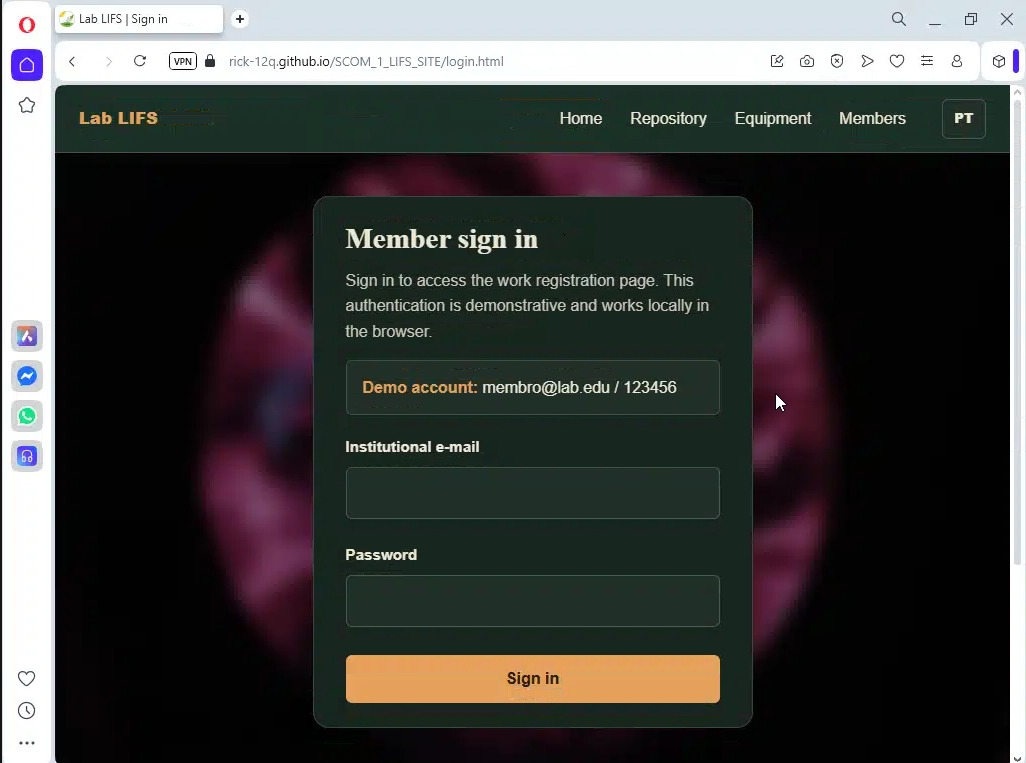
\includegraphics[width=\linewidth,height=0.23\textheight,keepaspectratio]{2-imagens/opera}
		\caption{Opera}
		\label{fig:opera}
	\end{subfigure}
	
	\caption{Testes de compatibilidade do site em diferentes navegadores.\\ \centering Fonte: O autor, 2026.}
	\label{fig:compatibilidade-navegadores}
\end{figure}




